\textbf{$\ket{\psi^+}=\frac{1}{\sqrt{2}} (\ket{01}+\ket{10})$} \vspace{.3cm}

\begin{quote}
    \begin{minted}[fontsize=\small, linenos, frame=single]{python}
estado_inicial = [0,1]
circuito_bell3 = QuantumCircuit(2)
circuito_bell3.initialize(estado_inicial,1)
circuito_bell3.h(0)
circuito_bell3.cx(0,1)                #cx: controlled x
circuito_bell3.measure_all()
circuito_bell3.draw('mpl')
    \end{minted}
    \vspace{.3cm}
    \begin{center}
        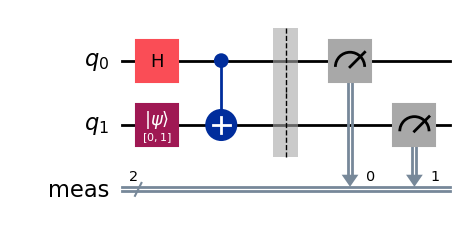
\includegraphics[height=3.3cm]{src/Img/3.2.png}
    \end{center}

    En este caso, usamos la combinación inicial $\ket{01}$:

    \begin{align*}
        \hat{C_x}\hat{H}\ket{01}
        = \hat{C_x} \left( \frac{1}{\sqrt{2}} (\ket{01}+\ket{11}) \right)
        = \frac{1}{\sqrt{2}} (\ket{01}+\ket{10})
    \end{align*}

    Podemos comprobar sacando el statevector, recordando que la base es $00,01,10,00$.
    \vspace{.5cm}

    \begin{center}
        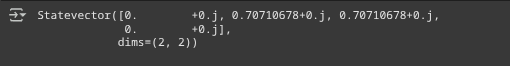
\includegraphics[width=.8\textwidth]{src/Img/3.2.r.png}
    \end{center}
\end{quote}
\vspace{.5cm}
